\documentclass[letterpaper, 11pt]{extarticle}
% \usepackage{fontspec}

% ==================================================

% document parameters
% \usepackage[spanish, mexico, es-lcroman]{babel}
\usepackage[english]{babel}
\usepackage[margin = 1in]{geometry}

% ==================================================

% Packages for math
\usepackage{mathrsfs}
\usepackage{amsfonts}
\usepackage{amsmath}
\usepackage{amsthm}
\usepackage{amssymb}
\usepackage{physics}
\usepackage{dsfont}
\usepackage{esint}

% ==================================================

% Packages for writing
\usepackage{enumerate}
\usepackage[shortlabels]{enumitem}
\usepackage{framed}
\usepackage{csquotes}

% ==================================================

% Miscellaneous packages
\usepackage{float}
\usepackage{tabularx}
\usepackage{xcolor}
\usepackage{multicol}
\usepackage{subcaption}
\usepackage{caption}
\captionsetup{format = hang, margin = 10pt, font = small, labelfont = bf}

% Citation
\usepackage[round, authoryear]{natbib}

% Hyperlinks setup
\usepackage{hyperref}
\definecolor{links}{rgb}{0.36,0.54,0.66}
\hypersetup{
   colorlinks = true,
    linkcolor = black,
     urlcolor = blue,
    citecolor = blue,
    filecolor = blue,
    pdfauthor = {Author},
     pdftitle = {Title},
   pdfsubject = {subject},
  pdfkeywords = {one, two},
  pdfproducer = {LaTeX},
   pdfcreator = {pdfLaTeX},
   }
\usepackage{titlesec}
\usepackage[many]{tcolorbox}
\usepackage{amsmath}
% Adjust spacing after the chapter title
\titlespacing*{\chapter}{0cm}{-2.0cm}{0.50cm}
\titlespacing*{\section}{0cm}{0.50cm}{0.25cm}

% Indent 
\setlength{\parindent}{0pt}
\setlength{\parskip}{1ex}

% --- Theorems, lemma, corollary, postulate, definition ---
% \numberwithin{equation}{section}

\newtcbtheorem[]{problem}{Problem}%
    {enhanced,
    colback = black!5, %white,
    colbacktitle = black!5,
    coltitle = black,
    boxrule = 0pt,
    frame hidden,
    borderline west = {0.5mm}{0.0mm}{black},
    fonttitle = \bfseries\sffamily,
    breakable,
    before skip = 3ex,
    after skip = 3ex
}{problem}

\tcbuselibrary{skins, breakable}

% --- You can define your own color box. Just copy the previous \newtcbtheorm definition and use the colors of yout liking and the title you want to use.
% --- Basic commands ---
%   Euler's constant
\newcommand{\eu}{\mathrm{e}}

%   Imaginary unit
\newcommand{\im}{\mathrm{i}}

%   Sexagesimal degree symbol
\newcommand{\grado}{\,^{\circ}}

% --- Comandos para álgebra lineal ---
% Matrix transpose
\newcommand{\transpose}[1]{{#1}^{\mathsf{T}}}

%%% Comandos para cálculo
%   Definite integral from -\infty to +\infty
\newcommand{\Int}{\int\limits_{-\infty}^{\infty}}

%   Indefinite integral
\newcommand{\rint}[2]{\int{#1}\dd{#2}}

%  Definite integral
\newcommand{\Rint}[4]{\int\limits_{#1}^{#2}{#3}\dd{#4}}

%   Dot product symbol (use the command \bigcdot)
\makeatletter
\newcommand*\bigcdot{\mathpalette\bigcdot@{.5}}
\newcommand*\bigcdot@[2]{\mathbin{\vcenter{\hbox{\scalebox{#2}{$\m@th#1\bullet$}}}}}
\makeatother

%   Hamiltonian
\newcommand{\Ham}{\hat{\mathcal{H}}}

%   Trace
\renewcommand{\Tr}{\mathrm{Tr}}

% Christoffel symbol of the second kind
\newcommand{\christoffelsecond}[4]{\dfrac{1}{2}g^{#3 #4}(\partial_{#1} g_{#2 #4} + \partial_{#2} g_{#1 #4} - \partial_{#4} g_{#1 #2})}

% Riemann curvature tensor
\newcommand{\riemanncurvature}[5]{\partial_{#3} \Gamma_{#4 #2}^{#1} - \partial_{#4} \Gamma_{#3 #2}^{#1} + \Gamma_{#3 #5}^{#1} \Gamma_{#4 #2}^{#5} - \Gamma_{#4 #5}^{#1} \Gamma_{#3 #2}^{#5}}

% Covariant Riemann curvature tensor
\newcommand{\covariantriemanncurvature}[5]{g_{#1 #5} R^{#5}{}_{#2 #3 #4}}

% Ricci tensor
\newcommand{\riccitensor}[5]{g_{#1 #5} R^{#5}{}_{#2 #3 #4}}
\usepackage{listings}

\begin{document}
\begin{Large}
    \textsf{\textbf{37005 Fundamentals of Derivative Security Pricing}}
    
    Group assignment
\end{Large}

\vspace{2ex}

\textsf{\textbf{Group 1 Students:}}

\text{Quoc Thai Tran}, \href{mailto:quocthai.tran@student.uts.edu.au}{\texttt{quocthai.tran@student.uts.edu.au}}

\text{Hayoung Lee}, \href{mailto:hayoung.lee-2@student.uts.edu.au}{\texttt{hayoung.lee-2@student.uts.edu.au}}

\text{Alexis Cullet}, \href{mailto:alexisdidier.cullet@student.uts.edu.au}{\texttt{alexisdidier.cullet@student.uts.edu.au}}

\text{Ziqi Zhou}, \href{mailto:ziqi.zhou-3@student.uts.edu.au}{\texttt{ziqi.zhou-3@student.uts.edu.au}}

\textsf{\textbf{Professor:}}

\text{Erik Schlögl}, \href{mailto:Erik.Schlogl@uts.edu.au}{\texttt{Erik.Schlogl@uts.edu.au}}

\section*{Task 1}

The objective of this is to estimate the Dividend Discount Factor $D(0, T)$ and the Zero Coupon Bond Price $B(0, T)$ for various maturities $T$. These factors are derived from the relationship between the call and put option prices using the Put-Call parity formula. The task involves using mid-prices of call and put options, minimizing the squared deviation from the theoretical relationship. 
\vspace{1ex}
We can define a function for the squared deviation from the relationship.
\begin{equation}
g(d_i ,b_i,K_{i,j},T_i)=((d_i S_0 - b_i K_{i,j}) - (C(K_{i,j},T_i)-P(K_{i,j},T_i)))^2
\end{equation}
where \(T_i\) denotes the \(i\)-th maturity, and \(K_{i,j}\) denotes the \(j\)-th strike for the \(i\)-th maturity and \(d_i\) and \(b_i\) represent \(D(0,T_i)\) and \(B(0,T_i)\), respectively, for the \(i\)-th maturity.
\vspace{1ex}
We can find \(d_i\) and \(b_i\) such that
\[\min_{d_i,b_i} \sum_{j=1}^{n_i} g(d_i ,b_i,K_{i,j},T_i)\]
where \(n_i\) denotes the number of strikes for the \(i\)-th maturity.
The results are as follows.
\begin{figure}[H]
    \centering
    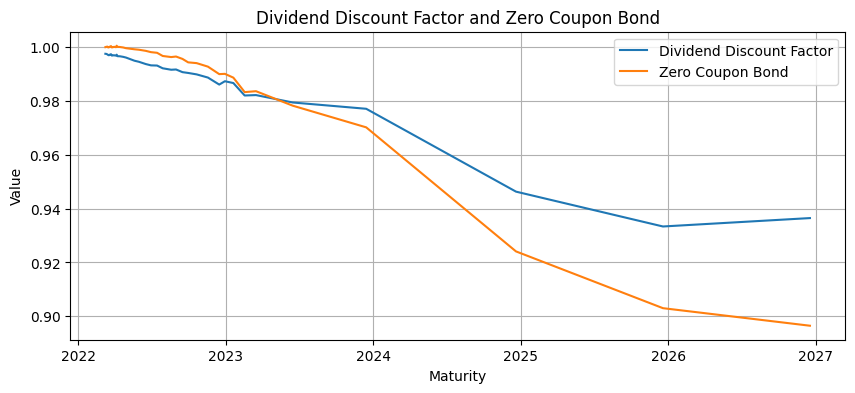
\includegraphics[width=1\linewidth]{discount_dividend.png}
\end{figure}
\begin{table}
\centering
\caption{Task 1 Result}
\label{tab:task1}
\begin{tabular}{l l l}   
Maturity & Dividend Discount Factor & Zero Coupon Bond \\
2022-03-09 & 0.9975 & 1.0000 \\
2022-03-11 & 0.9975 & 1.0001 \\
2022-03-14 & 0.9973 & 1.0002 \\
2022-03-16 & 0.9970 & 0.9998 \\
2022-03-18 & 0.9969 & 0.9999 \\
2022-03-21 & 0.9973 & 1.0002 \\
2022-03-23 & 0.9973 & 1.0003 \\
2022-03-25 & 0.9968 & 0.9999 \\
2022-03-28 & 0.9969 & 1.0000 \\
2022-03-30 & 0.9970 & 1.0001 \\
2022-03-31 & 0.9969 & 1.0000 \\
2022-04-01 & 0.9969 & 1.0001 \\
2022-04-04 & 0.9968 & 1.0000 \\
2022-04-06 & 0.9972 & 1.0005 \\
2022-04-08 & 0.9966 & 1.0001 \\
2022-04-14 & 0.9966 & 1.0000 \\
2022-04-22 & 0.9964 & 0.9998 \\
2022-04-29 & 0.9961 & 0.9996 \\
2022-05-20 & 0.9949 & 0.9992 \\
2022-05-31 & 0.9945 & 0.9990 \\
2022-06-17 & 0.9937 & 0.9986 \\
2022-06-30 & 0.9932 & 0.9981 \\
2022-07-15 & 0.9931 & 0.9979 \\
2022-07-29 & 0.9921 & 0.9967 \\
2022-08-19 & 0.9916 & 0.9963 \\
2022-08-31 & 0.9917 & 0.9965 \\
2022-09-16 & 0.9907 & 0.9956 \\
2022-09-30 & 0.9904 & 0.9943 \\
2022-10-21 & 0.9898 & 0.9940 \\
2022-11-18 & 0.9887 & 0.9927 \\
2022-12-16 & 0.9861 & 0.9899 \\
2022-12-30 & 0.9873 & 0.9900 \\
2023-01-20 & 0.9866 & 0.9886 \\
2023-02-17 & 0.9820 & 0.9833 \\
2023-03-17 & 0.9822 & 0.9836 \\
2023-06-16 & 0.9794 & 0.9782 \\
2023-12-15 & 0.9771 & 0.9702 \\
2024-12-20 & 0.9463 & 0.9241 \\
2025-12-19 & 0.9334 & 0.9030 \\
2026-12-18 & 0.9365 & 0.8965 \\

\end{tabular}

\end{table}
\newpage
\section*{Task 2}

Let us examine the case of options on the bid price and ask price.
First, for each maturity, extract the data such that a strike is the closest to the forward price, which is defined as:
\[\min_{K_i}\left|K_i - S(0)\frac{D(0,T_i)}{B(0,T_i)}\right|  \]

In the given data set of options on S\&P 500, it has information on the bid price of the call and put options. We can choose data about the call or put option price that have the greater spread. Using the chosen price, we can extract the information of a piecewise constant function that we set up until the corresponding maturity. 
\vspace{1ex}
Let us look at this in a more mathematical way.
The dynamic of the S\&P 500 is as follows.
\[dS(u)=S(u)((r(u)-q(u))du+\sigma(u)dW(u))\]
We defined the piecewise constant function of volatility as
\[\sigma(t)=c_i \;\text{when}\;T_i\leq t<T_{i+1} \]
Then,
\begin{align*}
\log S(T) &= \log S(0) + \int_0^T \left(r(u)-q(u)-\frac{1}{2}\sigma^2(u)\right)du+     \int_0^T \sigma(u)dW(u)\\
&= \log \left( S(0)\right)+\int_0^Tr(u)du-\int_0^Tq(u)du -\frac{1}{2}\int_0^T\sigma^2(u)du +\int_0^T \sigma(u)dW(u)\\
&= \log \left( S(0)\right)-\log \left( B(0,T)\right) +\log \left( D(0,T)\right) -\frac{1}{2}\int_0^T\sigma^2(u)du +\int_0^T \sigma(u)dW(u)\\
&= \log \left( S(0)\frac{D(0,T)}{B(0,T)}\right)-\frac{1}{2}\sum_{i=0}^{n-1}\int_{T_i}^{T_{i+1}} \sigma^2(u)du+\sum_{i=0}^{n-1}\int_{T_i}^{T_{i+1}} \sigma(u)dW(u)\\
&= \log \left( S(0)\frac{D(0,T)}{B(0,T)}\right)-\frac{1}{2}\sum_{i=0}^{n-1}\int_{T_i}^{T_{i+1}} {c_i}^2du+\sum_{i=0}^{n-1}\int_{T_i}^{T_{i+1}} {c_i}dW(u)\\
&= \log \left( S(0)\frac{D(0,T)}{B(0,T)}\right)-\frac{1}{2}\sum_{i=0}^{n-1} {c_i}^2\int_{T_i}^{T_{i+1}}du+\sum_{i=0}^{n-1}{c_i}\int_{T_i}^{T_{i+1}} dW(u)\\
&= \log \left( S(0)\frac{D(0,T)}{B(0,T)}\right)-\frac{1}{2}\sum_{i=0}^{n-1} {c_i}^2(T_{i+1}-T_{i})+\sum_{i=0}^{n-1} c_i (W(T_{i+1})-W(T_{i}))\\
\end{align*}
\begin{align*}
    T_{n}=T \quad and \quad T_0=0
\end{align*}

We can see
\[log S(T) \sim N \left(\log \left( S(0)\frac{D(0,T)}{B(0,T)}\right)-\frac{1}{2}\sum_{i=0}^{n-1} {c_i}^2(T_{i+1}-T_{i}),\sum_{i=0}^{n-1} {c_i}^2(T_{i+1}-T_{i})\right)\]

In case of the call option, the Black-Scholes model is as follows.
\[C_i(0)=S(0)D(0,T_i)\mathcal{N}(d_{1,i})-K_iB(0,T_i)\mathcal{N}(d_{2,i})\]
\[P_i(0)=-S(0)D(0,T_i)\mathcal{N}(-d_{1,i})+K_iB(0,T_i)\mathcal{N}(-d_{2,i})\]
\vspace{1ex}
where \[ d_{1,i}=\frac{\log(\frac{S(0)}{K_i})+\log(\frac{D(0,T_i)}{B(0,T_i)})+\frac{1}{2}\chi_i}{\sqrt{\chi_i}}
\]
\[d_{2,i}=d_{1,i}-\sqrt{\chi_i}\]
\[\chi_i=\sum_{j=0}^{i-1}c_j^2(T_{j+1}-T_{j}) \;\text{, }\; \chi_0=0\]

Then we can obtain the \(c_i\) for each maturity numerically by:
\[c_i^2(T_{i+1}-T_{i})=\chi_i-\chi_{i-1}\]

We can have the quantity of\
\(c_i^2(T_{i+1}-T_{i})\) by taking the first-order discrete difference.
Finally, we can calibrate each \(c_i\) from every quantity of
\(c_i^2(T_{i+1}-T_{i})\). In this manner, we can obtain both the bid and the ask volatility \(c_i\).
\vspace{1ex}
The results are as follows.
\begin{figure}[h]
    \centering
    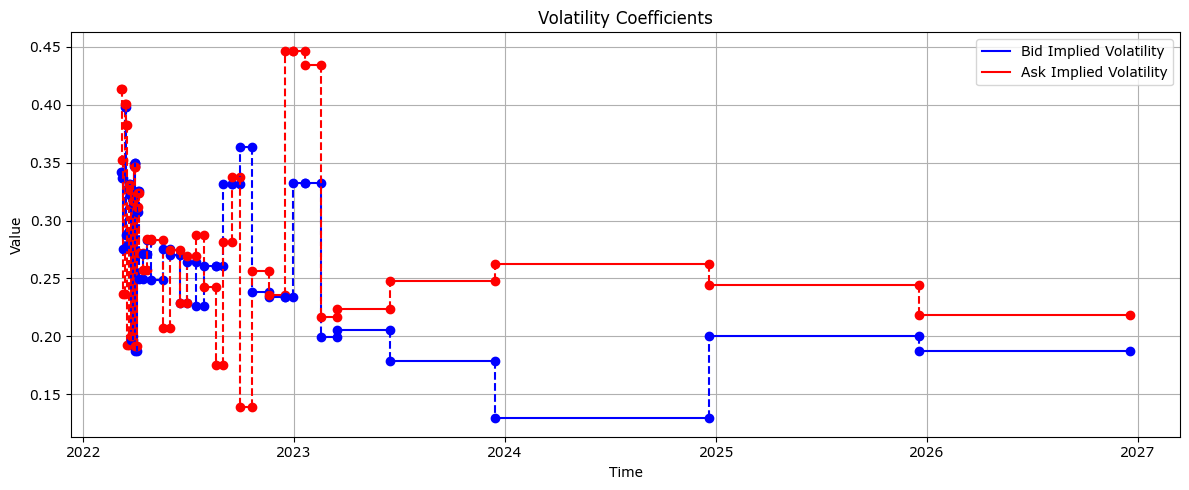
\includegraphics[width=1\linewidth]{task_2.png}
\end{figure}

As there exist pairs \(\chi_i<\chi_{i-1}\), which leads to the negative value of \({c_i}^2\) (which are unsolvable), we set \(c_i=c_{i-1}\). There are total 4 \(c_i\) of the bid price that fall into the situation and 1 \(c_i\) of the ask price that fall into the situation.

\begin{itemize}
    \item Maturity: 2022-08-31 00:00:00 Type: Bid Set to previous value:  0.26039029315491835
    \item Maturity: 2022-09-30 00:00:00 Type: Bid Set to previous value:  0.3318401251067233
    \item Maturity: 2022-12-30 00:00:00 Type: Bid Set to previous value:  0.2336100086129915
    \item Maturity: 2023-01-20 00:00:00 Type: Ask Set to previous value:  0.4465175941958699
    \item Maturity: 2023-02-17 00:00:00 Type: Bid Set to previous value:  0.3325796624075029
\end{itemize}

\begin{table}
\centering
\caption{Task 2 Result}
\label{tab:task2}
\begin{tabular}{l l l}   
Maturity & Bid Implied Volatility & Ask Implied Volatility \\
2022-03-09 & 0.3419 & 0.4133 \\
2022-03-11 & 0.3364 & 0.3519 \\
2022-03-14 & 0.2754 & 0.2368 \\
2022-03-16 & 0.3982 & 0.4006 \\
2022-03-18 & 0.2878 & 0.3825 \\
2022-03-21 & 0.2777 & 0.1923 \\
2022-03-23 & 0.3316 & 0.3310 \\
2022-03-25 & 0.3224 & 0.3260 \\
2022-03-28 & 0.1969 & 0.2004 \\
2022-03-30 & 0.3150 & 0.3164 \\
2022-03-31 & 0.3469 & 0.3484 \\
2022-04-01 & 0.3500 & 0.3465 \\
2022-04-04 & 0.1877 & 0.1916 \\
2022-04-06 & 0.3070 & 0.3113 \\
2022-04-08 & 0.3253 & 0.3237 \\
2022-04-14 & 0.2495 & 0.2716 \\
2022-04-22 & 0.2712 & 0.2576 \\
2022-04-29 & 0.2834 & 0.2844 \\
2022-05-20 & 0.2486 & 0.2834 \\
2022-05-31 & 0.2758 & 0.2073 \\
2022-06-17 & 0.2706 & 0.2742 \\
2022-06-30 & 0.2292 & 0.2289 \\
2022-07-15 & 0.2646 & 0.2691 \\
2022-07-29 & 0.2262 & 0.2877 \\
2022-08-19 & 0.2604 & 0.2428 \\
2022-08-31 & 0.2604 & 0.1751 \\
2022-09-16 & 0.3318 & 0.2816 \\
2022-09-30 & 0.3318 & 0.3377 \\
2022-10-21 & 0.3634 & 0.1389 \\
2022-11-18 & 0.2383 & 0.2563 \\
2022-12-16 & 0.2336 & 0.2356 \\
2022-12-30 & 0.2336 & 0.4465 \\
2023-01-20 & 0.3326 & 0.4465 \\
2023-02-17 & 0.3326 & 0.4338 \\
2023-03-17 & 0.1998 & 0.2164 \\
2023-06-16 & 0.2053 & 0.2241 \\
2023-12-15 & 0.1791 & 0.2476 \\
2024-12-20 & 0.1293 & 0.2629 \\
2025-12-19 & 0.2008 & 0.2445 \\
2026-12-18 & 0.1870 & 0.2182 \\

\end{tabular}

\end{table}


\section*{Task 3}
The client's payoff at time T
\[max(S(0)e^{gT},S(0)^\alpha S(T)^{1-\alpha})\]
Denote \(V(g)\) The price formula at time 0 with guarantee return of \(g\). Then,
\begin{align*}
V(g) &= B(0,T)\mathbb{E}[ max(S(0)e^{gT},S(0)^\alpha S(T)^{1-\alpha}] \\
&= B(0,T) \mathbb{E}[ S(0)e^{gT}\mathbb{I}_{S(0)e^{gT}>S(0)^\alpha S(T)^{1-\alpha}}]+B(0,T) \mathbb{E}[S(0)^\alpha S(T)^{1-\alpha}\mathbb{I}_{S(0)e^{gT}<S(0)^\alpha S(T)^{1-\alpha}}] \\
&=  B(0,T)S(0)e^{gT}\mathbb{E}[ \mathbb{I}_{S(0)e^{gT}>S(0)^\alpha S(T)^{1-\alpha}}]+ B(0,T)S(0)^\alpha \mathbb{E}[S(T)^{1-\alpha}\mathbb{I}_{S(0)e^{gT}<S(0)^\alpha S(T)^{1-\alpha}}]
\end{align*}
We know the distribution of index on S\&P 500.
\[log S(T) \sim N \left(log \left( S(0)\frac{D(0,T)}{B(0,T)}\right)-\frac{1}{2}\sum_{i=0}^{n-1} {c_i}^2(T_{i+1}-T_{i}),\sum_{i=0}^{n-1} {c_i}^2(T_{i+1}-T_{i})\right)\]
First term, 
\begin{align*}
  \mathbb{E}[ \mathbb{I}_{S(0)e^{gT}>S(0)^\alpha S(T)^{1-\alpha})}]&= \mathbb{P}\left[ {\log S(T)<\log S(0)+\frac{gT}{(1-\alpha)} }\right]\\
  &=\Phi\left(\frac{\frac{gT}{(1-\alpha)}-log \left( \frac{D(0,T)}{B(0,T)}\right)+\frac{1}{2}\sum_{i=0}^{n-1} {c_i}^2(T_{i+1}-T_{i})}{\sqrt{\sum_{i=0}^{n-1} {c_i}^2(T_{i+1}-T_{i})}}\right)
\end{align*}

In the second term, \( S(T)^{1-\alpha}\) can be removed by changing the measure.
Let \(Z(T)\) denote Radon-Nikodym derivative,
\[Z(T)= \frac{S(T)^{1-\alpha}}{S(0)^{1-\alpha}} C\]
where \(C\) is deterministic and \(Z(T)\) is martingale under \(\mathbb{P}\). Then, we must have \(Z(T)\) be:
\begin{align*}
    Z(T) &= Exp\left[-\frac{1}{2}\int_0^T (1-\alpha)^2\sigma(u)^2du+\int_0^T(1-\alpha)\sigma(u)dW(u)\right] \\
    &= Exp\left[-\frac{(1-\alpha)^2}{2}\int_0^T\sigma(u)^2du+(1-\alpha)\int_0^T\sigma(u)dW(u)\right] \\
    &= Exp\left[-\frac{(1-\alpha)^2}{2}\sum_{i=0}^{n-1}{c_i}^2(T_{i+1}-T_{i})+(1-\alpha)\sum_{i=0}^{n-1} c_i (W(T_{i+1})-W(T_{i}))\right]
\end{align*}
From the dynamics of the index, we have:
\[\frac{S(T)^{1-\alpha}}{S(0)^{1-\alpha}}=\left(\frac{D(0,T)}{B(0,T)}\right)^{1-\alpha}Exp\left[-\frac{(1-\alpha)}{2}\sum_{i=0}^{n-1} {c_i}^2(T_{i+1}-T_{i})+(1-\alpha)\sum_{i=0}^{n-1} c_i (W(T_{i+1})-W(T_{i}))\right]\]
Then,
\begin{multline*}
    Z(T)=C\left(\frac{D(0,T)}{B(0,T)}\right)^{1-\alpha}Exp\left[-(1-\alpha)\sum_{i=0}^{n-1} \frac{1}{2}{c_i}^2(T_{i+1}-T_{i})\right] 
    Exp\left[\frac{(1-\alpha)^2}{2}\sum_{i=0}^{n-1}{c_i}^2(T_{i+1}-T_{i})\right]\\
    Exp\left[-\frac{(1-\alpha)^2}{2}\sum_{i=0}^{n-1}{c_i}^2(T_{i+1}-T_{i})+(1-\alpha)\sum_{i=0}^{n-1} c_i W(T_{i+1}-T_{i})\right]
\end{multline*}

Hence,
\begin{align*}
    \frac{1}{C}&= \left(\frac{D(0,T)}{B(0,T)}\right)^{1-\alpha}    Exp\left[\left(\frac{(1-\alpha)^2}{2}-(1-\alpha)\right)\sum_{i=0}^{n-1} {c_i}^2(T_{i+1}-T_{i})\right] \\
    &=\left(\frac{D(0,T)}{B(0,T)}\right)^{1-\alpha}    Exp\left[\frac{\alpha^2-\alpha}{2}\sum_{i=0}^{n-1} {c_i}^2(T_{i+1}-T_{i})\right] 
\end{align*}
Then, we can write
\begin{align*}
    \mathbb{E}[S(T)^{1-\alpha}\mathbb{I}_{S(0)e^{gT}<S(0)^\alpha S(T)^{1-\alpha}}]&=\mathbb{E}_Q[\frac{1}{Z(T)}S(T)^{1-\alpha}\mathbb{I}_{S(0)e^{gT}<S(0)^\alpha S(T)^{1-\alpha}}]\\
    &=\mathbb{E}_Q[\frac{1}{C}\frac{S(0)^{1-\alpha}}{ S(T)^{1-\alpha}}S(T)^{1-\alpha}\mathbb{I}_{S(0)e^{gT}<S(0)^\alpha S(T)^{1-\alpha}}]\\
    &=\frac{S(0)^{1-\alpha}}{C}\mathbb{E}_Q[\mathbb{I}_{S(0)e^{gT}<S(0)^\alpha S(T)^{1-\alpha}}]\\
\end{align*}
Under Girsanov's Theorem,
\[W_Q(T_{i+1})-W_Q(T_i)=W(T_{i+1})-W(T_i)-(1-\alpha) c_i (T_{i+1}-T_i)\]
We can change the old measure to the new measure of \(S(T)\)'s dynamics. 
\begin{align*}
\log S(T) &= \log \left( S(0)\frac{D(0,T)}{B(0,T)}\right)-\frac{1}{2}\sum_{i=0}^{n-1} {c_i}^2(T_{i+1}-T_{i})\\
&+\sum_{i=0}^{n-1} c_i  \left[W_Q(T_{i+1})-W_Q(T_i)+(1-\alpha) c_i (T_{i+1}-T_i) \right]\\
&=\log \left( S(0)\frac{D(0,T)}{B(0,T)}\right)+(\frac{1}{2}-\alpha)\sum_{i=0}^{n-1} {c_i}^2(T_{i+1}-T_{i})+\sum_{i=0}^{n-1} c_i  (W_Q(T_{i+1})-W_Q(T_i))
\end{align*}

So we can see under \(Q\) measure,
\[log S(T) \sim N \left(log \left( S(0)\frac{D(0,T)}{B(0,T)}\right)+ (\frac{1}{2}-\alpha)\sum_{i=0}^{n-1}{c_i}^2(T_{i+1}-T_{i}),\sum_{i=0}^{n-1} {c_i}^2(T_{i+1}-T_{i})\right)\]
Then,
\begin{align*}
  \mathbb{E}_Q[\mathbb{I}_{S(0)e^{gT}<S(0)^\alpha S(T)^{1-\alpha}}]&= \mathbb{P}_Q[ \log S(T)>\log S(0)+\frac{gT}{(1-\alpha)} ]\\
  &=\Phi\left(\frac{-\frac{gT}{(1-\alpha)}+log \left( \frac{D(0,T)}{B(0,T)}\right)+(\frac{1}{2}-\alpha)\sum_{i=0}^{n-1} {c_i}^2(T_{i+1}-T_{i})}{\sqrt{\sum_{i=0}^{n-1} {c_i}^2(T_{i+1}-T_{i})}}\right)
\end{align*}
In conclusion,
\begin{align*}
    V(g,\alpha)&=B(0,T)S(0)e^{gT}\mathbb{E}[ \mathbb{I}_{S(0)e^{gT}>S(0)^\alpha S(T)^{1-\alpha}}]+ B(0,T)S(0)^\alpha \mathbb{E}[S(T)^{1-\alpha}\mathbb{I}_{S(0)e^{gT}<S(0)^\alpha S(T)^{1-\alpha}}]\\
    &=B(0,T)S(0)e^{gT}\Phi\left(h_1\right)+ S(0)B(0,T)^\alpha D(0,T)^{1-\alpha}    exp\left[\frac{\alpha^2-\alpha}{2}\sum_{i=0}^{n-1} {c_i}^2(T_{i+1}-T_{i})\right]\Phi\left(h_2\right)\\
\end{align*}
\begin{align*}
     h_1 &=\frac{\frac{gT}{(1-\alpha)}-log \left( \frac{D(0,T)}{B(0,T)}\right)+ \frac{1}{2}\sum_{i=0}^{n-1}{c_i}^2(T_{i+1}-T_{i})}{\sqrt{\sum_{i=0}^{n-1} {c_i}^2(T_{i+1}-T_{i})}}\\
   h_2 &=\frac{-\frac{gT}{(1-\alpha)}+log \left( \frac{D(0,T)}{B(0,T)}\right)+ (\frac{1}{2}-\alpha)\sum_{i=0}^{n-1}{c_i}^2(T_{i+1}-T_{i})}{\sqrt{\sum_{i=0}^{n-1} {c_i}^2(T_{i+1}-T_{i})}}
\end{align*}
\newpage
\section*{Task 4}

The enter date is 8 March 2022 and the maturity date is on 18 December 2026. The investment bank offers a client the contract which is the situation in which the bank is selling it and the client is purchasing it.
In the contract, the client only pays the amount of \(S(0)\) today. Then, the "fair" guarantee level \(g\) meaning the investment is fair such that
\[V(g,\alpha)=S(0)\]
When we calculate the value of this contract, we use the implied ask volatility as the ask price reflects the price which the buyer would pay in the transaction in the current market. 
In this procedure, because there exists an unsolvable \(c_i\), we can use the quantity of \(\chi_i=\sum_{i=0}^{n-1} {c_i}^2(T_{i+1}-T_{i})\) directly which we obtained from the asking price in Task 2.


The results are as follows.
\begin{table}[h]
    \centering
        \caption{Task 4 Results}
    \label{tab:task4_results}
    \begin{tabular}{|c|c|}
        \hline
        Share $\alpha$& Fair guarantee $g$\\
        \hline
        0.25 & -0.020276\\
        0.5 & 0.005402\\
        0.75 & 0.019758\\
        \hline
    \end{tabular}

\end{table}

To be much more seriously, we verify our pricing formula from task 3 by using task 4 results and Monte-Carlo method to estimate the discount expectation of the simulation of the payoff at the maturity under the  three given $\alpha$ and three corresponding guarantee level g computed previously. We generate a million random samples drawn from a standard normal distribution to finish this simulation. 

Define the payoff like what we done before.

\[max(S(0)e^{gT},S(0)^\alpha S(T)^{1-\alpha})\]

For $S(T)$ here.

\[S(T)=S(0)\frac{D(0,T)}{B(0,T)}Exp\left[\frac{-\chi_{n}}{2}+\sqrt{\chi_{n}}w\right]\]

On the above, $w$ represents samples drawn from a standard normal distribution.

The simulation results demonstrate that the values are clustered around the initial $S(0)$ value of 4170.7002. This observation lends credibility to the reliability of the previously established task 3 and task 4.

\begin{table}[h]
    \centering
        \caption{Task 4 Monte-Carlo simulation Results}
    \label{tab:task4_Monte_Carlo}
    \begin{tabular}{|c|c|c|}
        \hline
        Share $\alpha$& Fair guarantee $g$ & Simulation result\\
        \hline
        0.25 & -0.020276&4172.164097955495\\
        0.5 & 0.005402&4171.276516820223\\
        0.75 & 0.019758&4170.7833076323\\
        \hline
    \end{tabular}

\end{table}

\newpage
\section*{Task 5}
\subsection*{1. Minimizer target}
Let $\mathbf{X}$ denote the quantities (weights) of each instrument that we are buying (or selling) to super-hedging and is a vector, i.e.
\[\mathbf{X} = (w_{C_{S_1}}, \dots, w_{C_{S_N}}, w_{P_{S_1}}, \dots, w_{P_{S_N}}, w_{B(0,T)})^T, w_{(.)} \in \mathbb{R}\]

with $C_{S_n}$ (respectively, $P_{S_n}$) being a call (respectively a put) with strike $S_n$. Each weight can take any real value as we make the assumption that we can trade fractional assets. If the weight is negative, we consider that we are selling at the bid price. Conversely, if the weight is positive, we buy at the ask price.

Let $\mathbf{CP}$ denote the prices of each instrument that we are buying (or selling) in response to the position that we are going to take and be a vector, i.e.
\[\mathbf{CP}(\mathbf{X}) = ({C_{S_1}}(w_{C_{S_1}}), \dots, {C_{S_N}}(w_{C_{S_N}}), {P_{S_1}}(w_{P_{S_1}}), \dots, {P_{S_N}}(w_{P_{S_N}}), {B(0,T)})^T \\
\]
$$
{C_{S_i}}(w_{C_{S_i}}) =
\begin{cases} 
    (C_{S_i})_{ask} & \text{if } w_{C_{S_i}} \geq 0 \\ 
    (C_{S_i})_{bid} & \text{if } w_{C_{S_i}} < 0
\end{cases}
i \in [1,n]
$$
$$
{P_{S_i}}(w_{P_{S_i}}) =
\begin{cases} 
    (P_{S_i})_{ask} & \text{if } w_{P_{S_i}} \geq 0 \\ 
    (P_{S_i})_{bid} & \text{if } w_{P_{S_i}} < 0
\end{cases}
i \in [1,n]
$$

Then, our objective is to minimize the following functions with respect to the constraints that we are going to discuss in the next part.
\[
\min_{X}\mathbf{X}^T\mathbf{CP}(\mathbf{X})
\]

\subsection*{2. Constraints}
Let
\[G(\alpha, g, S(T))\]

denote the payoff of the option considered in Task 3. Let $$F(\mathbf{X}, S(T))$$ denote the payoff of the super hedge we are trying to build. We need to satisfy the condition that the payoff of the super hedge needs to be above the payoff of the option derived in Task 3. This can be done by looking at the sign of the minimum value of
\[F(\mathbf{X}, S(T)) - G(\alpha, g, S(T))\]

There are two ways in which we can find this sign. Our first option is to numerically solve a minimization problem. We can use \verb|scipy.optimize.minimize| on the difference of the payoff $F(\mathbf{X}, S(T)) - G(\alpha, g, S(T))$. Indeed, checking the sign of
$$(F(\mathbf{X})-G)(x_{min})$$
is enough to conclude on the super hedge payoff line being above the option payoff line.

However, in our experience, this is very hard to obtain for two reasons. The first one is that it is a very demanding process to optimize using \verb|scipy.optimize.minimize| every time we need to run the condition inside the already running minimizer of our payoff. The other reason being that the minimizer sometimes finds a local minimum and not the real minimum, giving us false positive constraints. Rather than proceeding with this approach, we decided to use a "Monte Carlo" approach. We uniformly look at the difference of payoffs for 2000 values of $S(T)$ between 0 and 20,000. This implies that we make the assumption that the index price will never exceed 20,000 by the expiration of the contract.
$$(F(\mathbf{X})-G)(x)\geq 0 \text{ with } x \in [0,20,000]$$
Any problem that arises from not satisfying the constraints of the super hedge due to this practice can be solved by adjusting the result after optimization.

The final constraints is found when we initially thought about narrowing the number of calls and puts to buy in $[-1,1]$ because the price of the contracts could change if we buy more than 1 unit, but we realized that the optimizer returned values in that range anyway. Furthermore, when looking at the given data, we saw that there was no bid position for the call options with strikes 8000, 8600 and 9000. Since then, the weight for this three position must be non-negative as we can't short it. So at the end, we have the constraints that 
\[-1 \leq w_{C_{S_i}} \leq 1 \text{ for \(S_i \notin \{8000, 8600, 9000\}\)}\]
\[0 \leq w_{C_{S_i}} \leq 1 \text{ for \(S_i \in \{8000, 8600, 9000\}\)} \]
\[-1 \leq w_{P_{S_i}} \leq 1\]
\subsection*{3. Result}
The result of cost and smallest difference in the payoff at the maturity is following:
\begin{table}[H]
    \centering
    \begin{tabular}{|c|c|c|c|}
        \hline
        $\alpha$& $0.25$ & $0.5$ & $0.75$ \\
        \hline
        Cost & $4,261.1096$& $4,200.7570$& $4,192.7819$\\
        \hline
        Payoff smallest difference & $0.0026$&$0.4983$ & $0.0922$\\
        \hline
    \end{tabular}
    \caption{Result of task 5}
    \label{tab:task_5_result}
\end{table}
The payoff graph is following:
\begin{figure}[H]
    \centering
    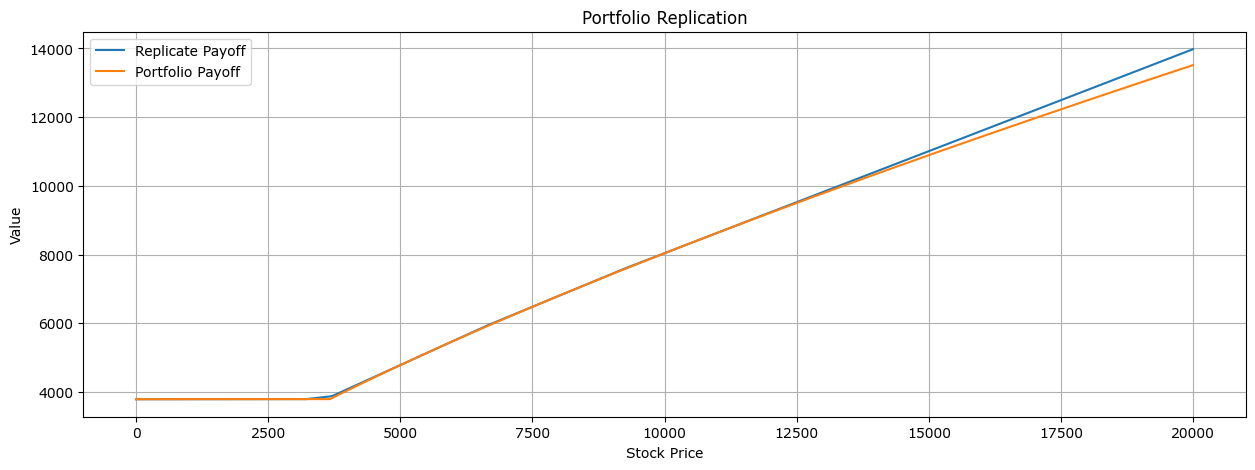
\includegraphics[width=1\linewidth]{output25.png}
    \caption{Payoff at $\alpha$=0.25}
    \label{tab:Payoff at 0.25}
\end{figure}
\begin{figure}[H]
    \centering
    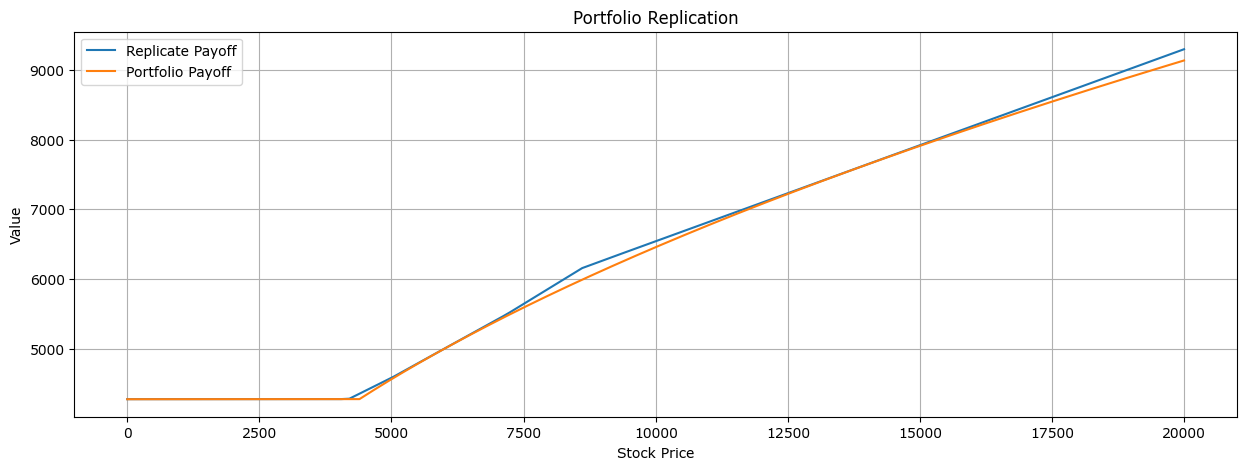
\includegraphics[width=1\linewidth]{output50.png}
    \caption{Payoff at $\alpha$=0.50}
    \label{tab:Payoff at 0.50}
\end{figure}
\begin{figure}[H]
    \centering
    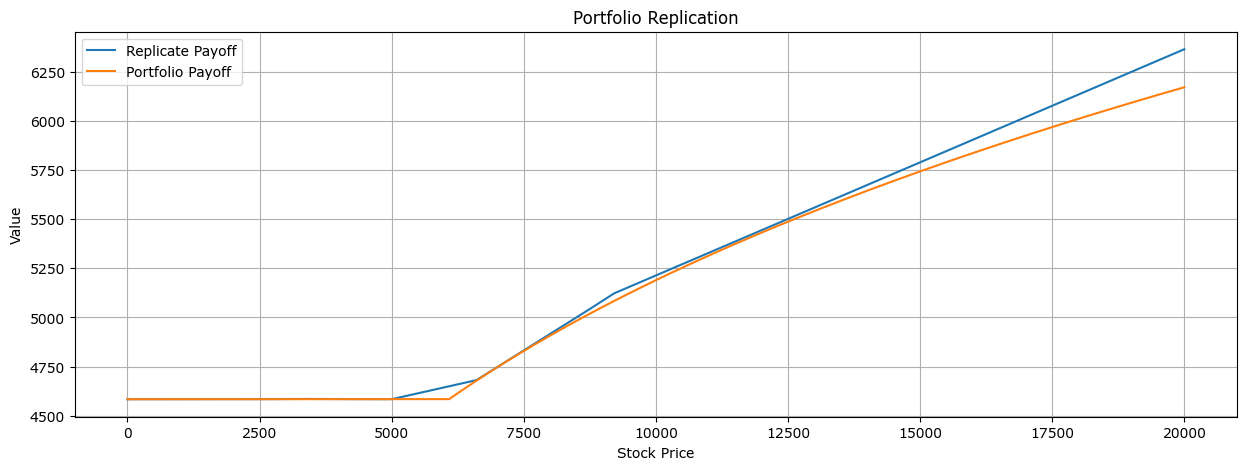
\includegraphics[width=1\linewidth]{output75.png}
    \caption{Payoff at $\alpha$=0.75}
    \label{tab:Payoff at 0.75}
\end{figure}
The result of position is as follows:
\begin{table}[H]
    \centering
    \begin{tabular}{|c|c|c|c|}
        \hline
        $\alpha $ & $0.25$ & $0.5$ & $0.75$ \\
        \hline
        \(w_{C_{2400}}\)  & $6.3489 \times 10^{-5}$  & $5.3519 \times 10^{-5}$  & $8.9341 \times 10^{-2}$ \\
        \(w_{C_{3200}}\)  & $1.0443 \times 10^{-1}$  & $8.0893 \times 10^{-7}$  & $-3.0302 \times 10^{-3}$ \\
        \(w_{C_{3700}}\)  & $5.3396 \times 10^{-1}$  & $4.0260 \times 10^{-4}$  & $1.1412 \times 10^{-6}$ \\
        \(w_{C_{4000}}\)  & $1.1093 \times 10^{-5}$  & $2.7115 \times 10^{-2}$  & $-3.0465 \times 10^{-5}$ \\
        \(w_{C_{4200}}\)  & $-7.3519 \times 10^{-7}$ & $1.5728 \times 10^{-1}$  & $-2.2914 \times 10^{-5}$ \\
        \(w_{C_{5000}}\)  & $1.2661 \times 10^{-5}$  & $4.2915 \times 10^{-2}$  & $5.9654 \times 10^{-2}$ \\
        \(w_{C_{6600}}\)  & $-4.2440 \times 10^{-4}$ & $3.6243 \times 10^{-3}$  & $1.0828 \times 10^{-1}$ \\
        \(w_{C_{7200}}\)  & $-5.2918 \times 10^{-7}$ & $4.3735 \times 10^{-2}$  & $-7.7216 \times 10^{-6}$ \\
        \(w_{C_{8000}}\)  & $2.5846 \times 10^{-7}$  & $1.7890 \times 10^{-6}$  & $2.2992 \times 10^{-6}$ \\
        \(w_{C_{8600}}\) & $2.5844 \times 10^{-7}$  & $1.6216 \times 10^{-6}$  & $1.8161 \times 10^{-6}$ \\
        \(w_{C_{9000}}\) & $2.5843 \times 10^{-7}$  & $1.6216 \times 10^{-6}$  & $1.6506 \times 10^{-6}$ \\
        \(w_{C_{9200}}\) & $-4.3981 \times 10^{-2}$ & $-1.8914 \times 10^{-6}$ & $-1.3903 \times 10^{-1}$ \\
        \(w_{P_{2400}}\) & $2.2821 \times 10^{-6}$  & $-2.3540 \times 10^{-5}$ & $-8.7404 \times 10^{-2}$ \\
        \(w_{P_{3200}}\) & $6.3247 \times 10^{-2}$  & $2.2255 \times 10^{-5}$  & $-7.4751 \times 10^{-5}$ \\
        \(w_{P_{3700}}\) & $1.2265 \times 10^{-6}$  & $2.5866 \times 10^{-6}$  & $6.3160 \times 10^{-4}$ \\
        \(w_{P_{4000}}\) & $2.6143 \times 10^{-6}$  & $3.5241 \times 10^{-4}$  & $-1.7796 \times 10^{-4}$ \\
        \(w_{P_{4200}}\) & $8.1452 \times 10^{-5}$  & $1.8938 \times 10^{-1}$  & $2.6602 \times 10^{-5}$ \\
        \(w_{P_{5000}}\) & $-3.5101 \times 10^{-6}$ & $-1.9238 \times 10^{-4}$ & $1.3039 \times 10^{-3}$ \\
        \(w_{P_{6600}}\) & $-6.3239 \times 10^{-2}$ & $-5.9622 \times 10^{-5}$ & $4.3119 \times 10^{-6}$ \\
        \(w_{P_{7200}}\) & $-2.6615 \times 10^{-5}$ & $-2.2122 \times 10^{-5}$ & $-5.9360 \times 10^{-7}$ \\
        \(w_{P_{8000}}\) & $-5.3908 \times 10^{-5}$ & $-8.4218 \times 10^{-5}$ & $3.5441 \times 10^{-6}$ \\
        \(w_{P_{8600}}\) & $-1.1664 \times 10^{-5}$ & $-1.8454 \times 10^{-1}$ & $5.5511 \times 10^{-3}$ \\
        \(w_{P_{9000}}\) & $1.0558 \times 10^{-6}$  & $-4.4340 \times 10^{-3}$ & $1.8929 \times 10^{-6}$ \\
        \(w_{P_{9200}}\) & $-1.3243 \times 10^{-6}$ & $-2.8096 \times 10^{-4}$ & $8.0144 \times 10^{-2}$ \\
        \(w_{B(0,T)}\) & $4.00074963 \times 10^{3}$   & $5.11559999 \times 10^{3}$   & $4.00058585 \times 10^{3}$ \\
        \hline
    \end{tabular}
    \caption{Positions for hedging with different $\alpha$ values}
    \label{tab:alpha_values}
\end{table}

From the result, we can see that our constraints are all met.
\begin{itemize}
    \item The constraints on the weights are meet
    \item The graph is diverge at the end compared to the target payoff
\end{itemize}
However, this result is not optimized yet as there exists the smallest difference that is different from 0. Since then we can reduce our cost more by performing the following adjustment.

\subsection*{4. Result adjustment}
Due to the problem mentioned above, we still can optimize our cost more by shifting down the hedge payoff line by offsetting the amount of zero coupon bond by the smallest difference. This practice won't affect the constraint that the hedging payoff is greater than the target payoff as we have run and calculated the smallest difference again on the adjusted positions. The result turns out that our smallest differences are all zeros. This is a sufficient and satisfying approximation, which, for us, is the best compromise between efficiency and precision. Also, graphically, we can see that the two payoffs at the end diverge, the payoff of the super hedge being a straight line above and increasing with a factor of $x$ while the payoff of the contract is a logarithmically increasing function below. Thus, the payoffs will never cross and the super hedge is satisfied at $+\infty$, even though 20,000 is already sufficiently unlikely for the S\&P 500 to reach in 2 years as it would represent a return of nearly 400$\%$ over that period.

\begin{table}[H]
    \centering
    \begin{tabular}{|c|c|c|c|}
        \hline
        $\alpha$& $0.25$ & $0.5$ & $0.75$ \\
        \hline
        Adjusted Cost & $4,261.1096$& $4,200.7570$& $4,192.7819$\\
        \hline
        Adjusted payoff smallest difference & $0$ & $0$ & $0$\\
        \hline
    \end{tabular}
    \caption{Result of task 5}
    \label{tab:adjusted_task_5_result}
\end{table}
The adjusted payoff graph is following:
\begin{figure}[H]
    \centering
    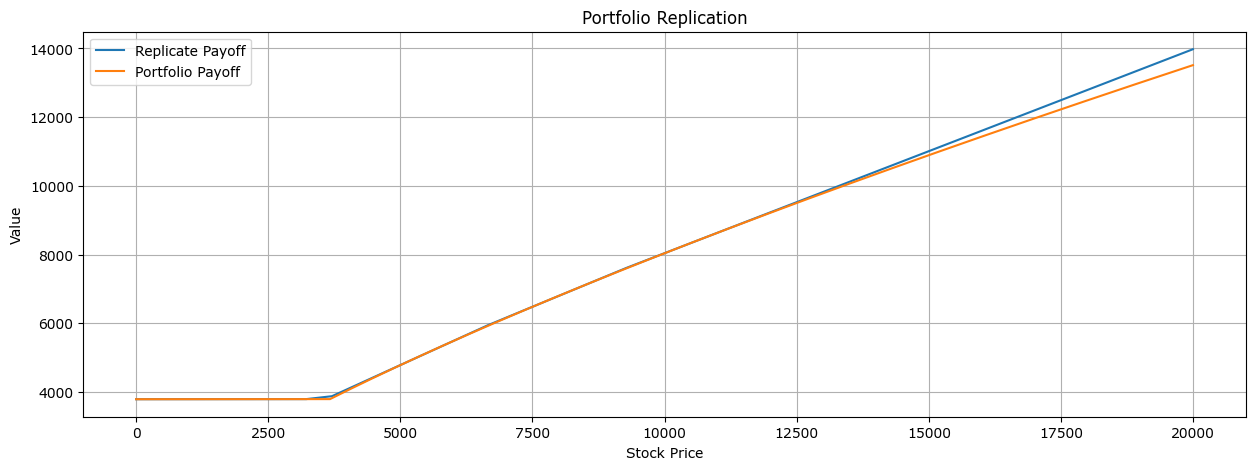
\includegraphics[width=1\linewidth]{adjusted_25.png}
    \caption{Adjusted Payoff at $\alpha$=0.25}
    \label{tab:Adjusted Payoff at 0.25}
\end{figure}
\begin{figure}[H]
    \centering
    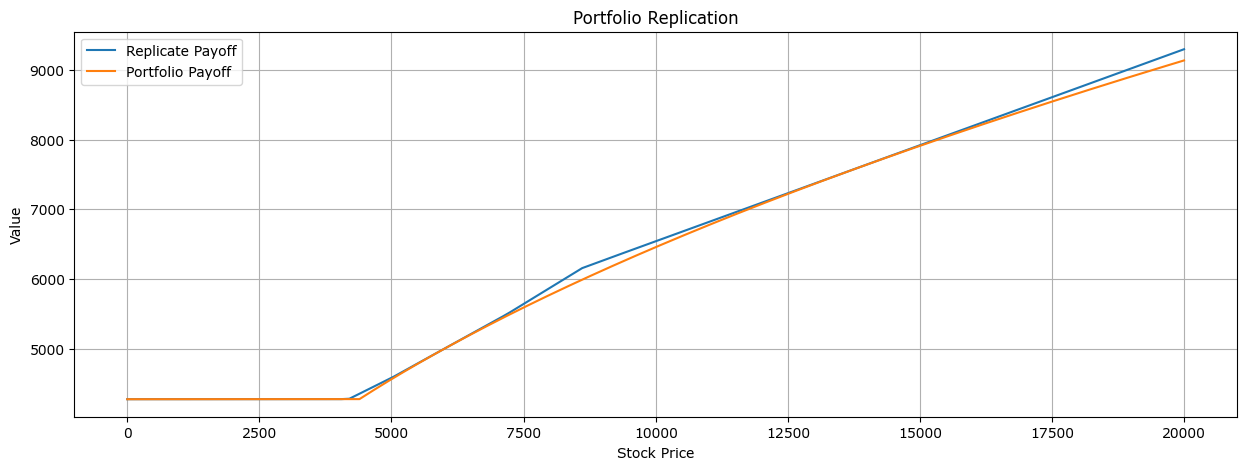
\includegraphics[width=1\linewidth]{adjusted_50.png}
    \caption{Adjusted Payoff at $\alpha$=0.50}
    \label{tab:Adjusted Payoff at 0.50}
\end{figure}
\begin{figure}[H]
    \centering
    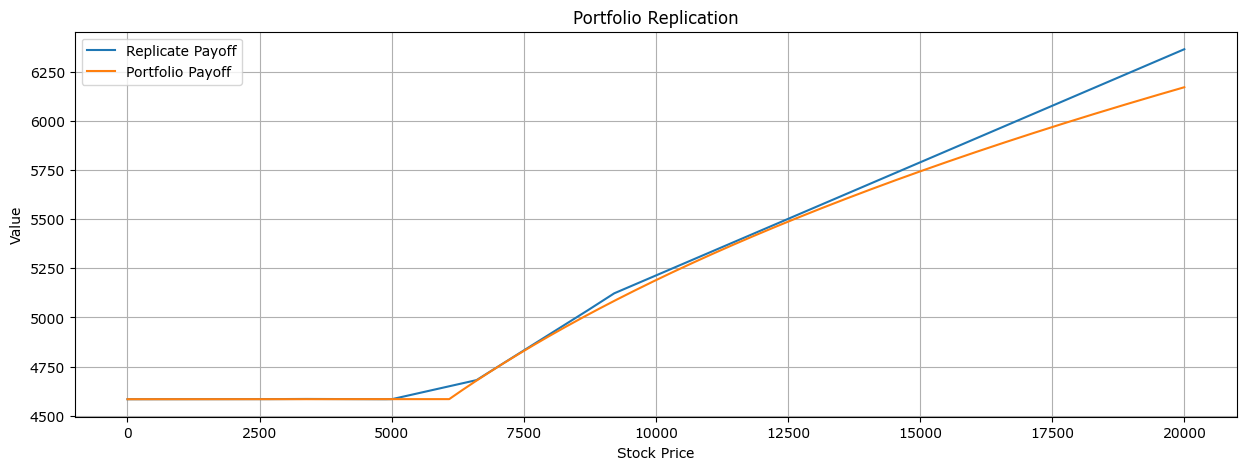
\includegraphics[width=1\linewidth]{adjusted_75.png}
    \caption{Adjusted Payoff at $\alpha$=0.75}
    \label{tab:Adjusted Payoff at 0.75}
\end{figure}

The result of adjusted position is following:
\begin{table}[H]
    \centering
    \begin{tabular}{|c|c|c|c|}
        \hline
        $\alpha$ & $0.25$ & $0.5$ & $0.75$ \\
        \hline
        \(w_{C_{2400}}\)  & $6.3489 \times 10^{-5}$  & $5.3519 \times 10^{-5}$  & $8.9341 \times 10^{-2}$ \\
        \(w_{C_{3200}}\)  & $1.0443 \times 10^{-1}$  & $8.0893 \times 10^{-7}$  & $-3.0302 \times 10^{-3}$ \\
        \(w_{C_{3700}}\)  & $5.3396 \times 10^{-1}$  & $4.0260 \times 10^{-4}$  & $1.1412 \times 10^{-6}$ \\
        \(w_{C_{4000}}\)  & $1.1093 \times 10^{-5}$  & $2.7115 \times 10^{-2}$  & $-3.0465 \times 10^{-5}$ \\
        \(w_{C_{4200}}\)  & $-7.3519 \times 10^{-7}$ & $1.5728 \times 10^{-1}$  & $-2.2914 \times 10^{-5}$ \\
        \(w_{C_{5000}}\)  & $1.2661 \times 10^{-5}$  & $4.2915 \times 10^{-2}$  & $5.9654 \times 10^{-2}$ \\
        \(w_{C_{6600}}\)  & $-4.2440 \times 10^{-4}$ & $3.6243 \times 10^{-3}$  & $1.0828 \times 10^{-1}$ \\
        \(w_{C_{7200}}\)  & $-5.2918 \times 10^{-7}$ & $4.3735 \times 10^{-2}$  & $-7.7216 \times 10^{-6}$ \\
        \(w_{C_{8000}}\)  & $2.5846 \times 10^{-7}$  & $1.7890 \times 10^{-6}$  & $2.2992 \times 10^{-6}$ \\
        \(w_{C_{8600}}\) & $2.5844 \times 10^{-7}$  & $1.6216 \times 10^{-6}$  & $1.8161 \times 10^{-6}$ \\
        \(w_{C_{9000}}\) & $2.5843 \times 10^{-7}$  & $1.6216 \times 10^{-6}$  & $1.6506 \times 10^{-6}$ \\
        \(w_{C_{9200}}\) & $-4.3981 \times 10^{-2}$ & $-1.8914 \times 10^{-6}$ & $-1.3903 \times 10^{-1}$ \\
        \(w_{P_{2400}}\) & $2.2821 \times 10^{-6}$  & $-2.3540 \times 10^{-5}$ & $-8.7404 \times 10^{-2}$ \\
        \(w_{P_{3200}}\) & $6.3247 \times 10^{-2}$  & $2.2255 \times 10^{-5}$  & $-7.4751 \times 10^{-5}$ \\
        \(w_{P_{3700}}\) & $1.2265 \times 10^{-6}$  & $2.5866 \times 10^{-6}$  & $6.3160 \times 10^{-4}$ \\
        \(w_{P_{4000}}\) & $2.6143 \times 10^{-6}$  & $3.5241 \times 10^{-4}$  & $-1.7796 \times 10^{-4}$ \\
        \(w_{P_{4200}}\) & $8.1452 \times 10^{-5}$  & $1.8938 \times 10^{-1}$  & $2.6602 \times 10^{-5}$ \\
        \(w_{P_{5000}}\) & $-3.5101 \times 10^{-6}$ & $-1.9238 \times 10^{-4}$ & $1.3039 \times 10^{-3}$ \\
        \(w_{P_{6600}}\) & $-6.3239 \times 10^{-2}$ & $-5.9622 \times 10^{-5}$ & $4.3119 \times 10^{-6}$ \\
        \(w_{P_{7200}}\) & $-2.6615 \times 10^{-5}$ & $-2.2122 \times 10^{-5}$ & $-5.9360 \times 10^{-7}$ \\
        \(w_{P_{8000}}\) & $-5.3908 \times 10^{-5}$ & $-8.4218 \times 10^{-5}$ & $3.5441 \times 10^{-6}$ \\
        \(w_{P_{8600}}\) & $-1.1664 \times 10^{-5}$ & $-1.8454 \times 10^{-1}$ & $5.5511 \times 10^{-3}$ \\
        \(w_{P_{9000}}\) & $1.0558 \times 10^{-6}$  & $-4.4340 \times 10^{-3}$ & $1.8929 \times 10^{-6}$ \\
        \(w_{P_{9200}}\) & $-1.3243 \times 10^{-6}$ & $-2.8096 \times 10^{-4}$ & $8.0144 \times 10^{-2}$ \\
        \(w_{B(0,T)}\) & $4.00074700 \times 10^{3}$   & $5.11510174 \times 10^{3}$   & $ 4.00049361 \times 10^{3}$ \\
        \hline
    \end{tabular}
    \caption{Adjusted Positions for hedging with different $\alpha$ values}
    \label{tab:adjusted alpha_values}
\end{table}

\newpage
\section*{Task 6}

In summary, the bank offers a client a contract guaranteeing an ex-dividend return of \(g\) in exchange for a share \(\alpha\). The \(g\) is determined fairly with the market data with respect to the corresponding \(\alpha\). From \ref{tab:summary_result}, we can see that as a share \(\alpha\) is decreasing, fair guarantee \(g\) is decreasing. It is understandable that the less the client exchanges for the share the less the bank guarantees the ex-dividend return. It can be interpreted that when \(\alpha\) is decreasing, the bank has more risk to the volatility of  \(S(T)\) at maturity as the payoff at maturity is \(max(S(0)e^{gT},S(0)^\alpha S(T)^{1-\alpha})\). It means the bank would protect the contract less, otherwise it creates arbitrage opportunities. In other words, the guarantee would be smaller to be fair.
In terms of the super hedge, at time 0 we have a loss from the super hedging as we have an investment amount \$4,170.7002 as the adjusted super hedge costs are all over the investment amount. However, at maturity we have positive payoffs almost surely. It can be confirmed with our graphs as well.
Furthermore, we can see that as a share \(\alpha\) is decreasing, the adjusted super hedge cost is increasing. It is understandable that as the bank is more at risk to \(S(T)\) with small \(\alpha\), we hedge this contract more expensively.

\begin{table}[H]
    \centering
    \begin{tabular}{|c|c|c|}
\hline
         $\alpha$
&  Fair guarantee $g$
& Adjusted super hedge cost
\\
\hline
         0.25 
&  -0.020276
& \$4,261.11
\\
         0.5 
&  0.005402
& \$4,200.31
\\
         0.75 &  0.019758& \$4,192.70\\
\hline
    \end{tabular}
    \caption{Summary}
    \label{tab:summary_result}
\end{table}

\begin{figure}[H]
    \centering
    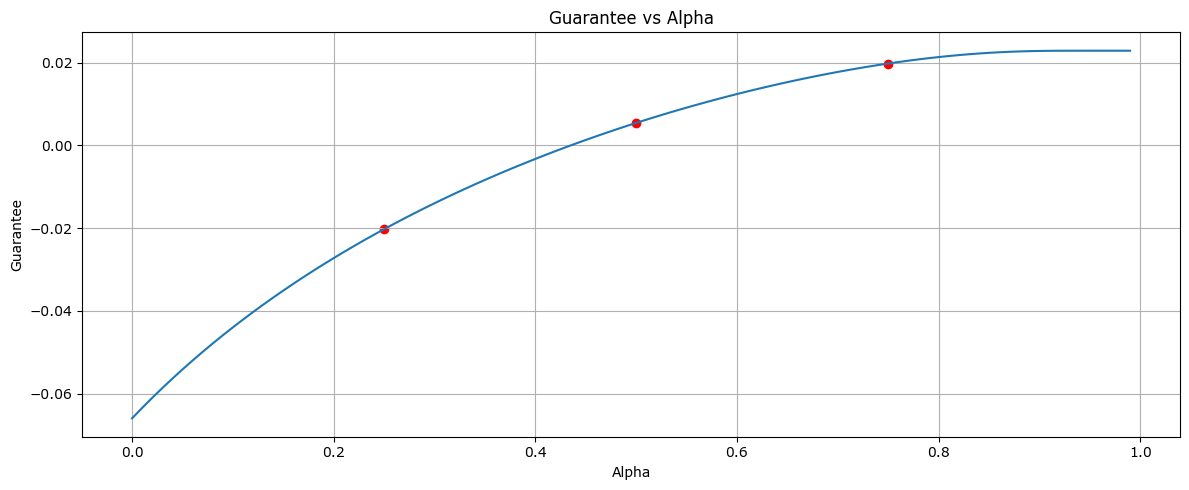
\includegraphics[width=1\linewidth]{task_6.png}
    \caption{Alpha vs Guarantee}
    \label{fig:alpha_guarantee}
\end{figure}

\end{document}